% appendix.tex -- 付録
\appendix
\chapter{追加実験結果}
追加実験の結果を以下に示す.
\begin{figure}[H]
    \centering
    \fbox{
        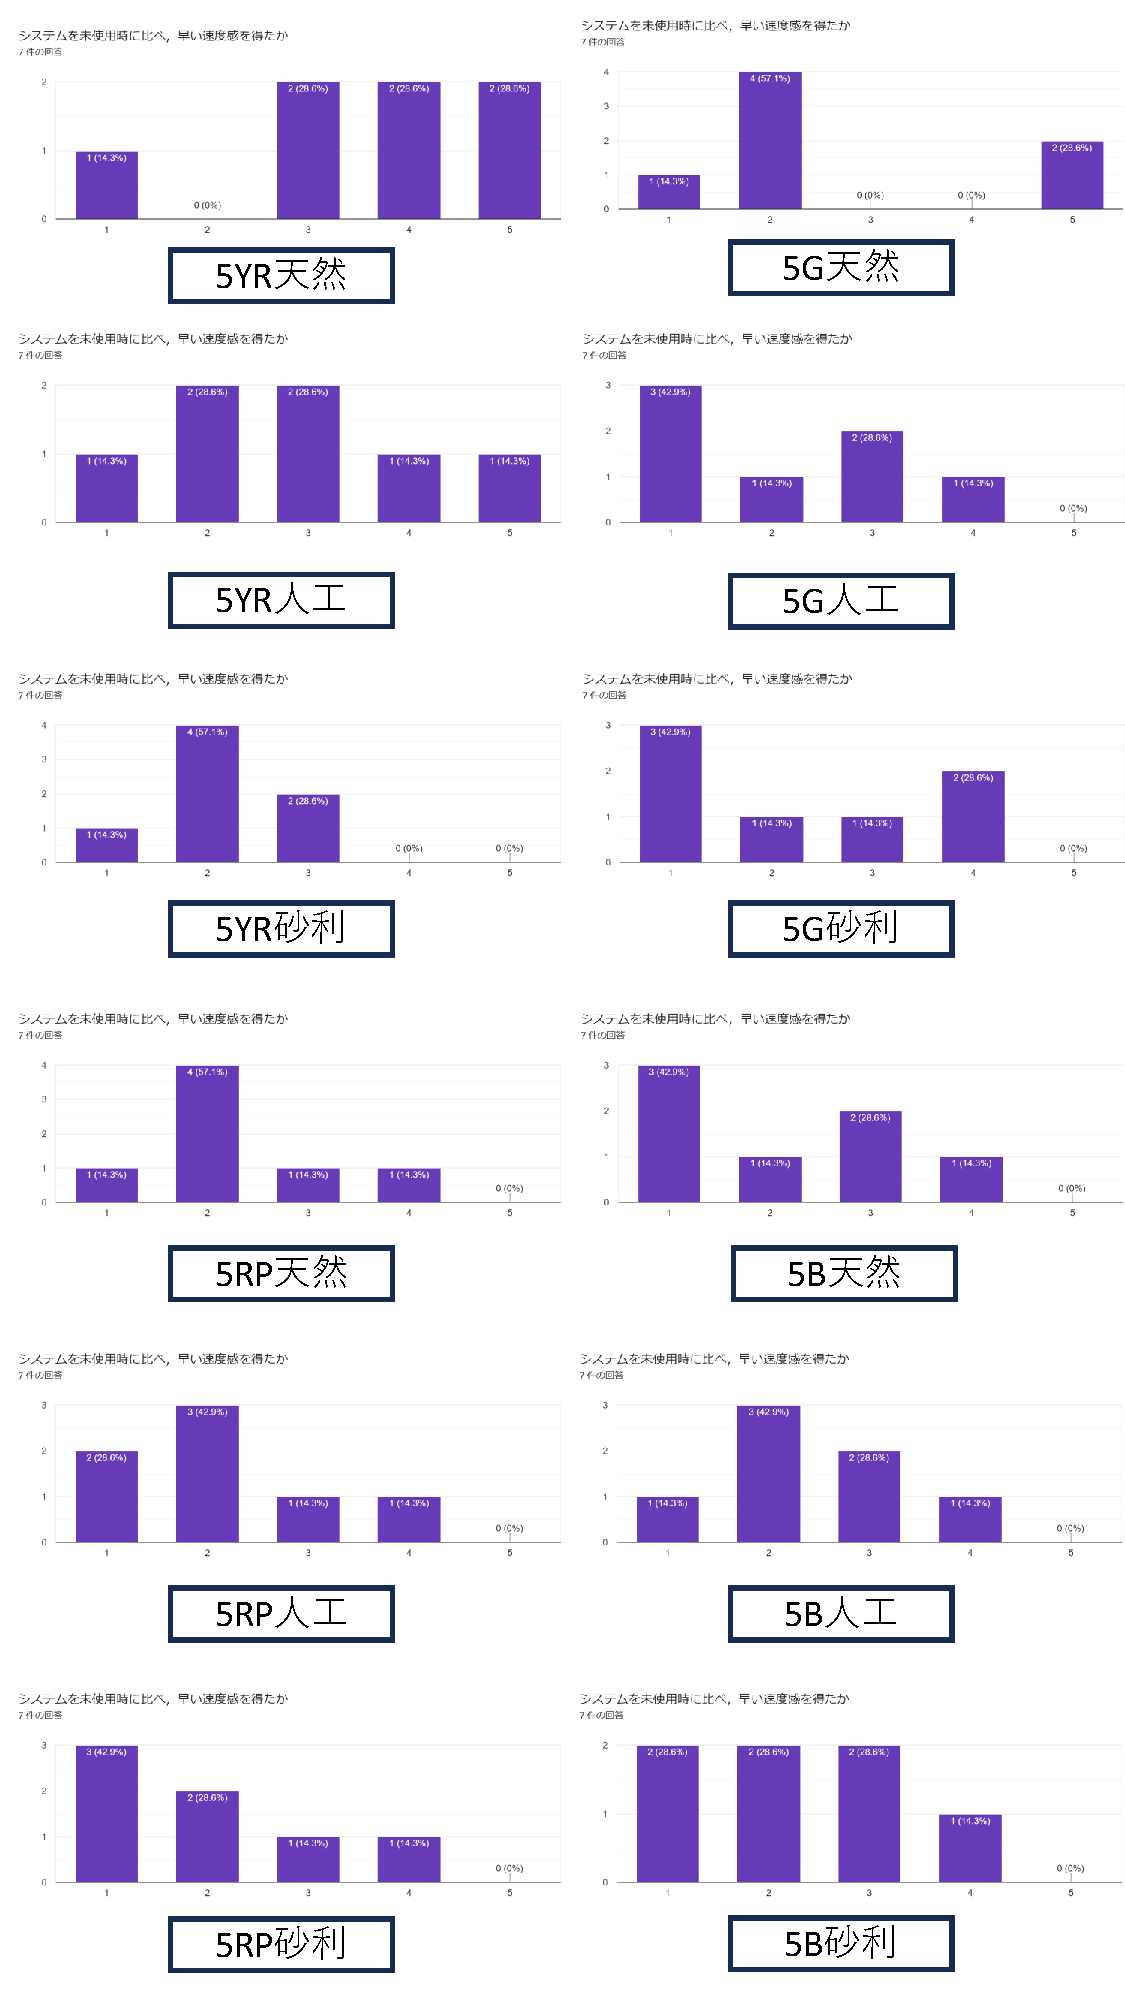
\includegraphics[width=0.8\linewidth]{fig/(前)faster.pdf}
    }
    \caption{バーチャル床が前から迫ってくることで早い速度感を得たかのアンケート結果}
    \label{fig:f1}
\end{figure}
\begin{figure}[H]
    \centering
    \fbox{
        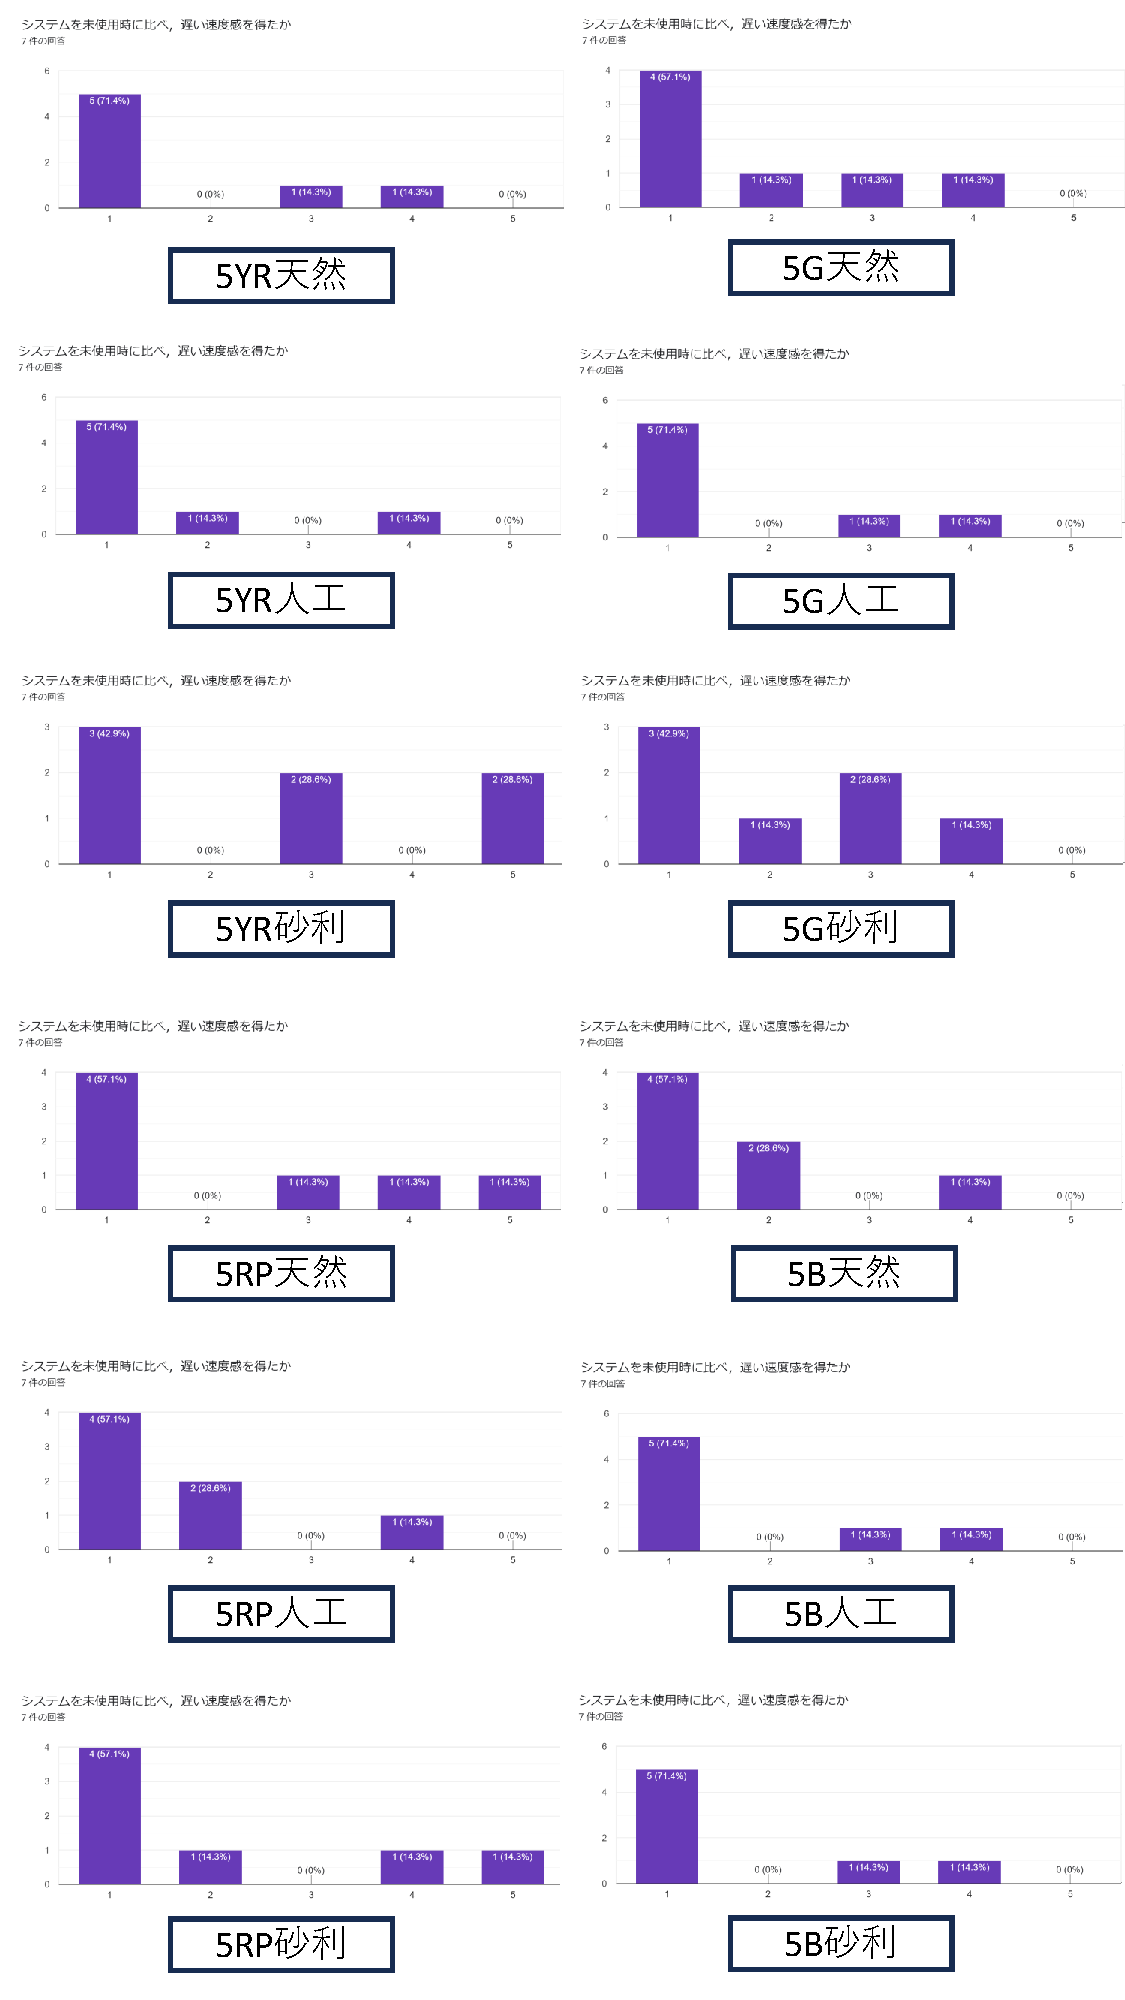
\includegraphics[width=0.8\linewidth]{fig/(前)slower.pdf}
    }
    \caption{バーチャル床が前から迫ってくることで遅い速度感を得たかのアンケート結果}
    \label{fig:f2}
\end{figure}
\begin{figure}[H]
    \centering
    \fbox{
        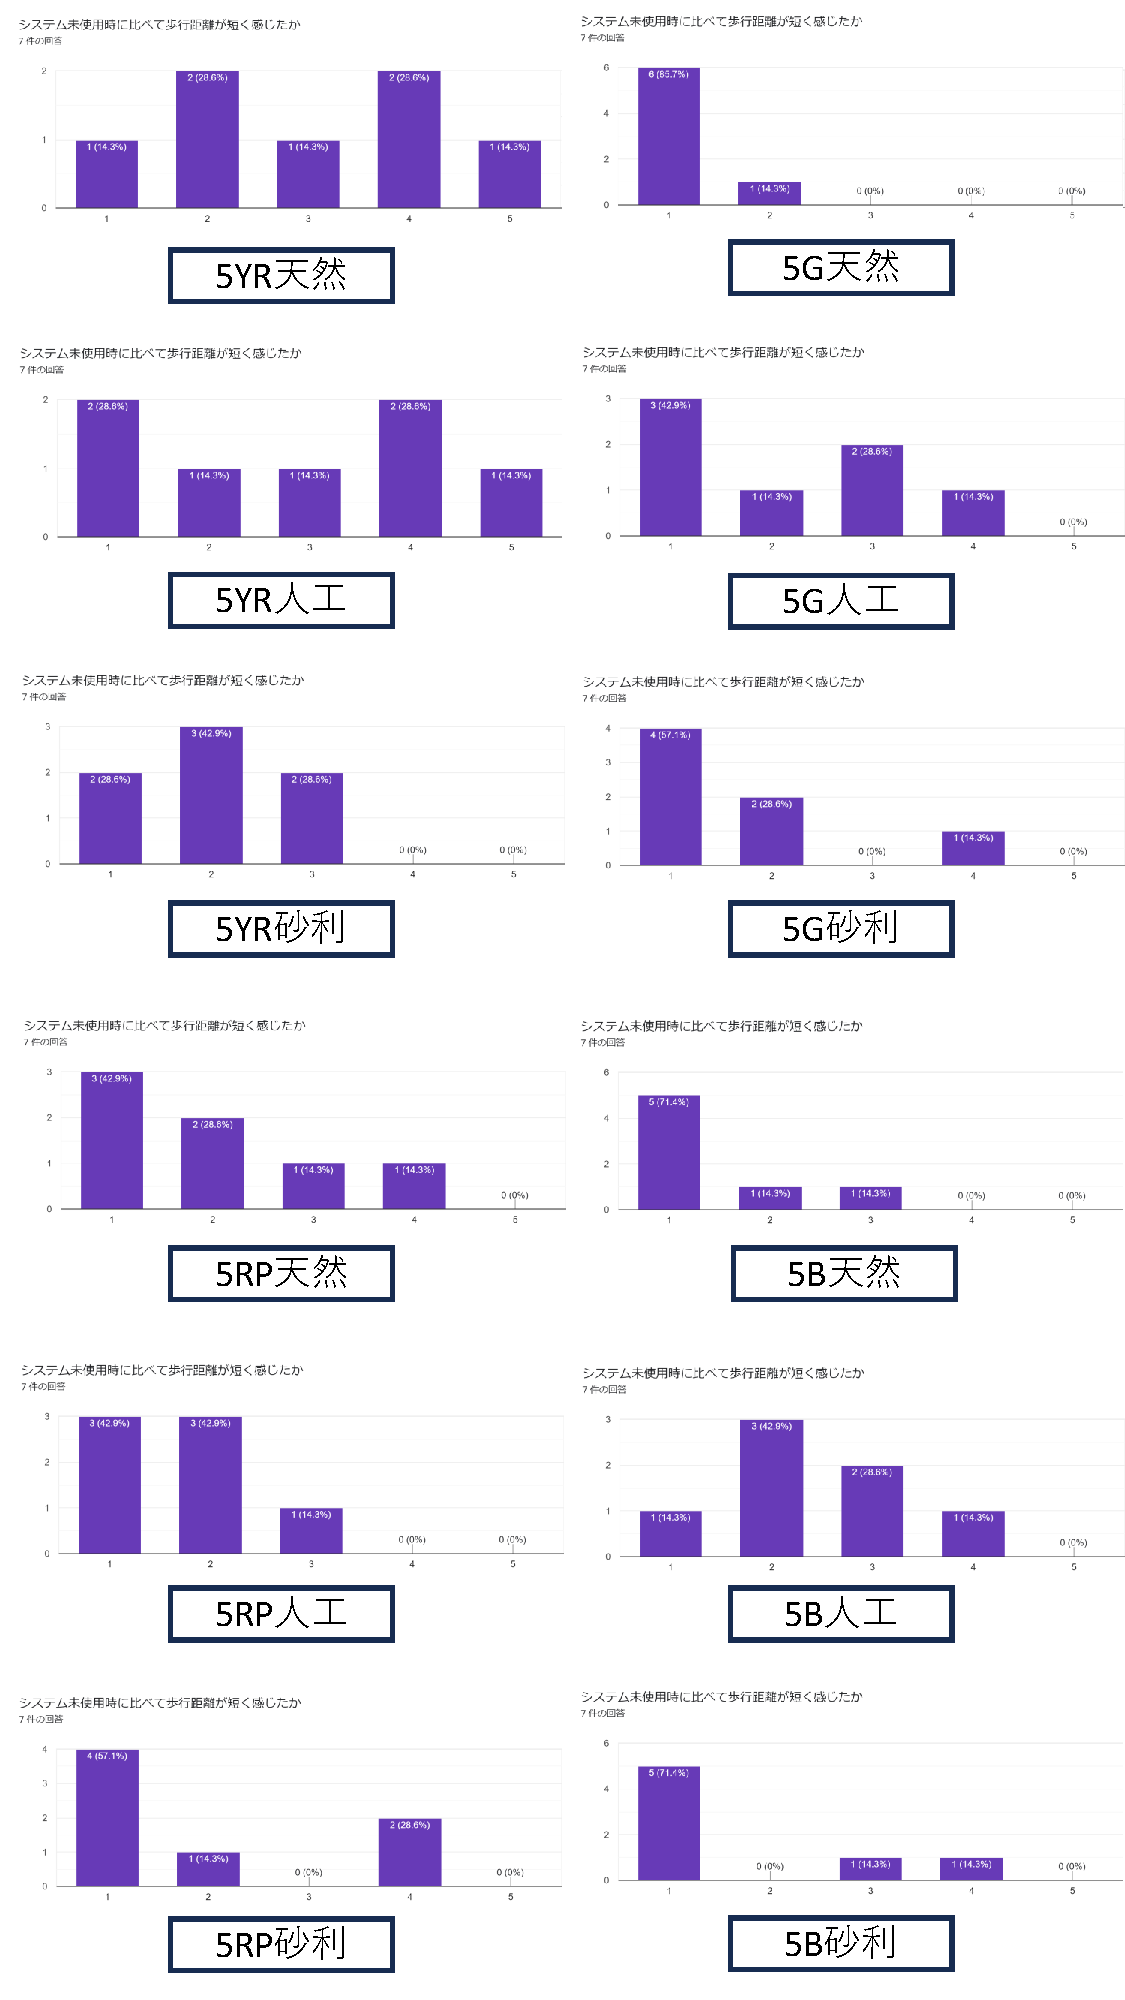
\includegraphics[width=0.8\linewidth]{fig/(前)shoater.pdf}
    }
    \caption{バーチャル床が前から迫ってくることで歩行距離が短く感じたかのアンケート結果}
    \label{fig:f3}
\end{figure}
\begin{figure}[H]
    \centering
    \fbox{
        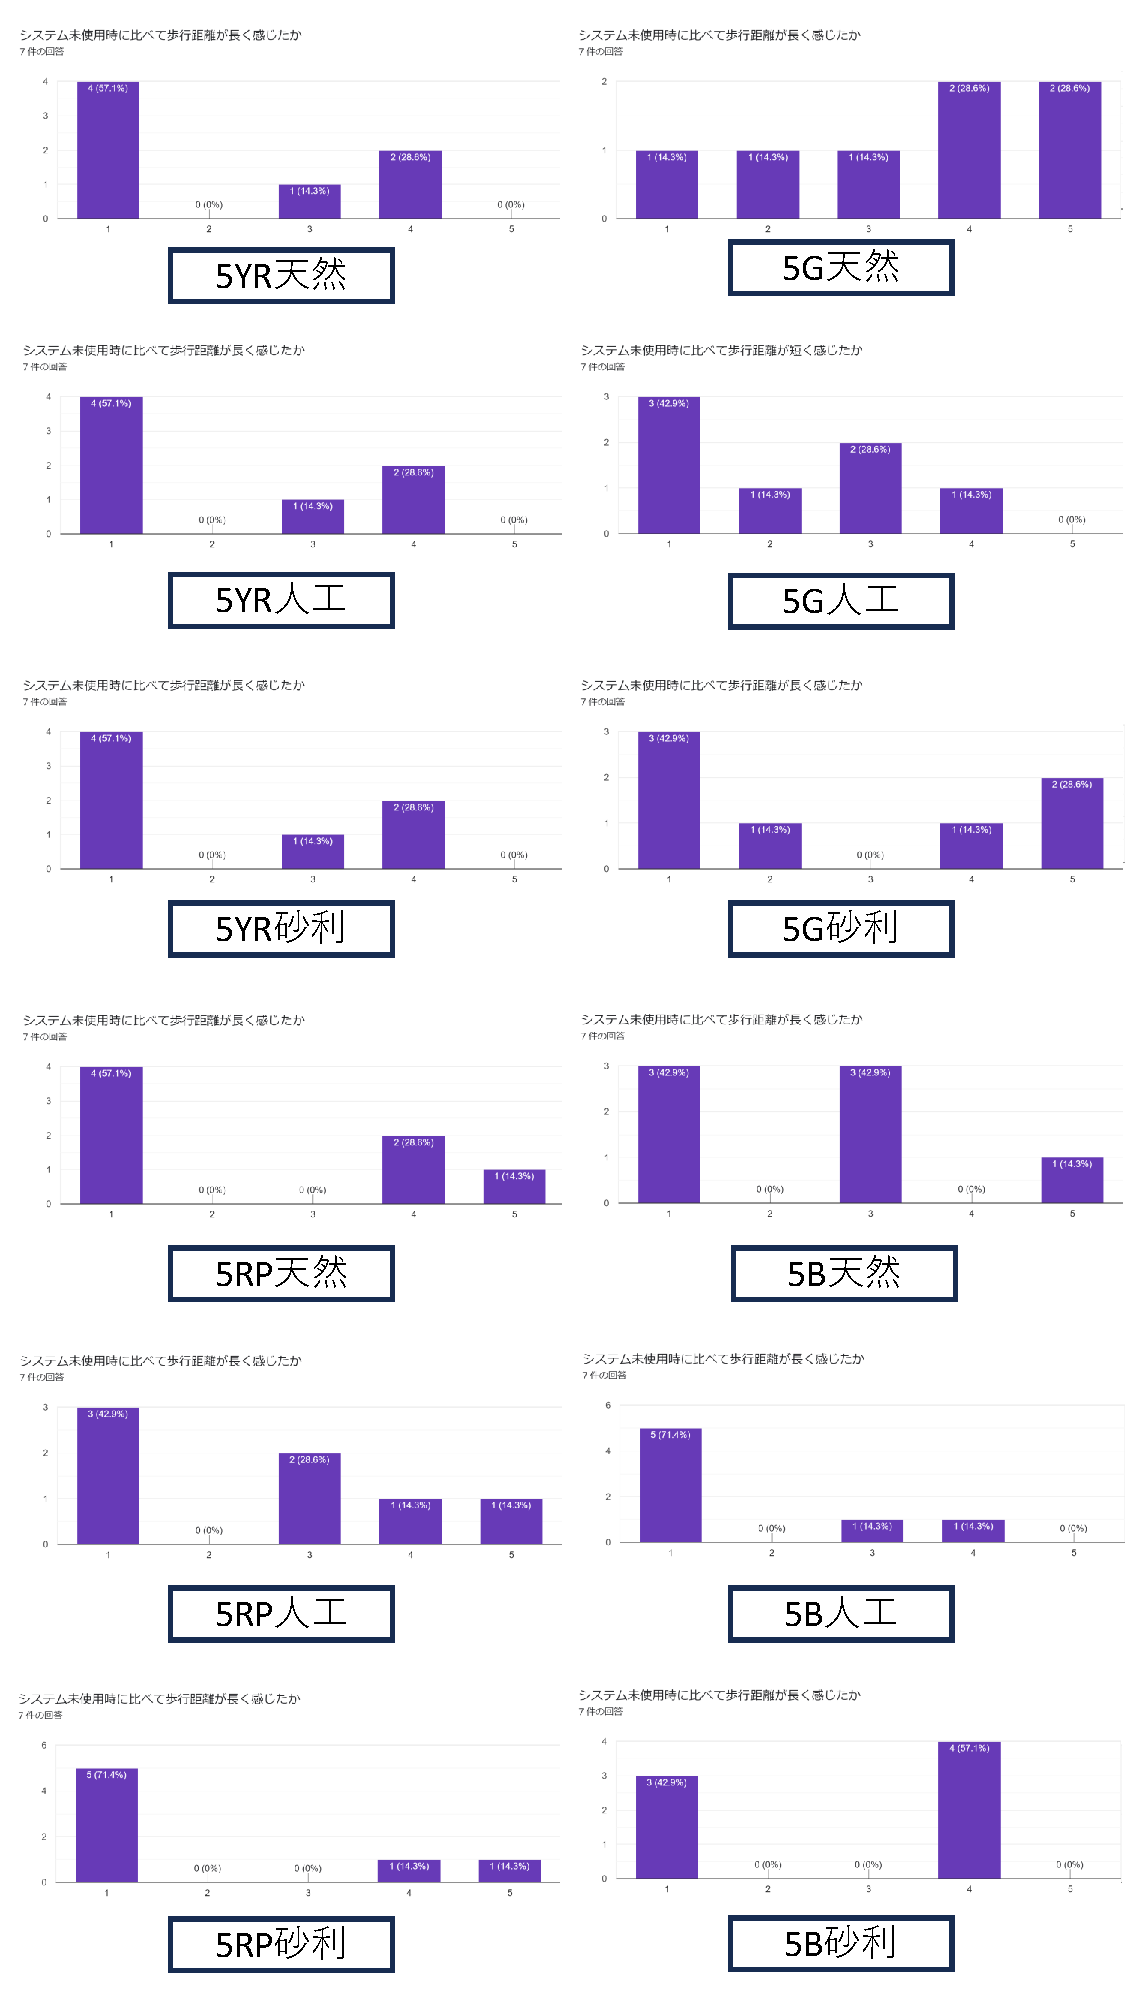
\includegraphics[width=0.8\linewidth]{fig/(前)longer.pdf}
    }
    \caption{バーチャル床が前から迫ってくることで歩行距離が長く感じたかのアンケート結果}
    \label{fig:f4}
\end{figure}
\begin{figure}[H]
    \centering
    \fbox{
        \includegraphics[width=0.8\linewidth]{fig/(後)faster.pdf}
    }
    \caption{バーチャル床が後ろから追い越してくることで早い速度感を得たかのアンケート結果}
    \label{fig:b1}
\end{figure}
\begin{figure}[H]
    \centering
    \fbox{
        \includegraphics[width=0.8\linewidth]{fig/(後)slower.pdf}
    }
    \caption{バーチャル床が後ろから追い越してくることで遅い速度感を得たかのアンケート結果}
    \label{fig:b2}
\end{figure}
\begin{figure}[H]
    \centering
    \fbox{
        \includegraphics[width=0.8\linewidth]{fig/(後)shoater.pdf}
    }
    \caption{バーチャル床が後ろから追い越してくることで歩行距離が短く感じたかのアンケート結果}
    \label{fig:b3}
\end{figure}
\begin{figure}[H]
    \centering
    \fbox{
        \includegraphics[width=0.8\linewidth]{fig/(後)longer.pdf}
    }
    \caption{バーチャル床が後ろから追い越してくることで歩行距離が長く感じたかのアンケート結果}
    \label{fig:b4}
\end{figure}

\begin{figure}[H]
    \centering
    \fbox{
        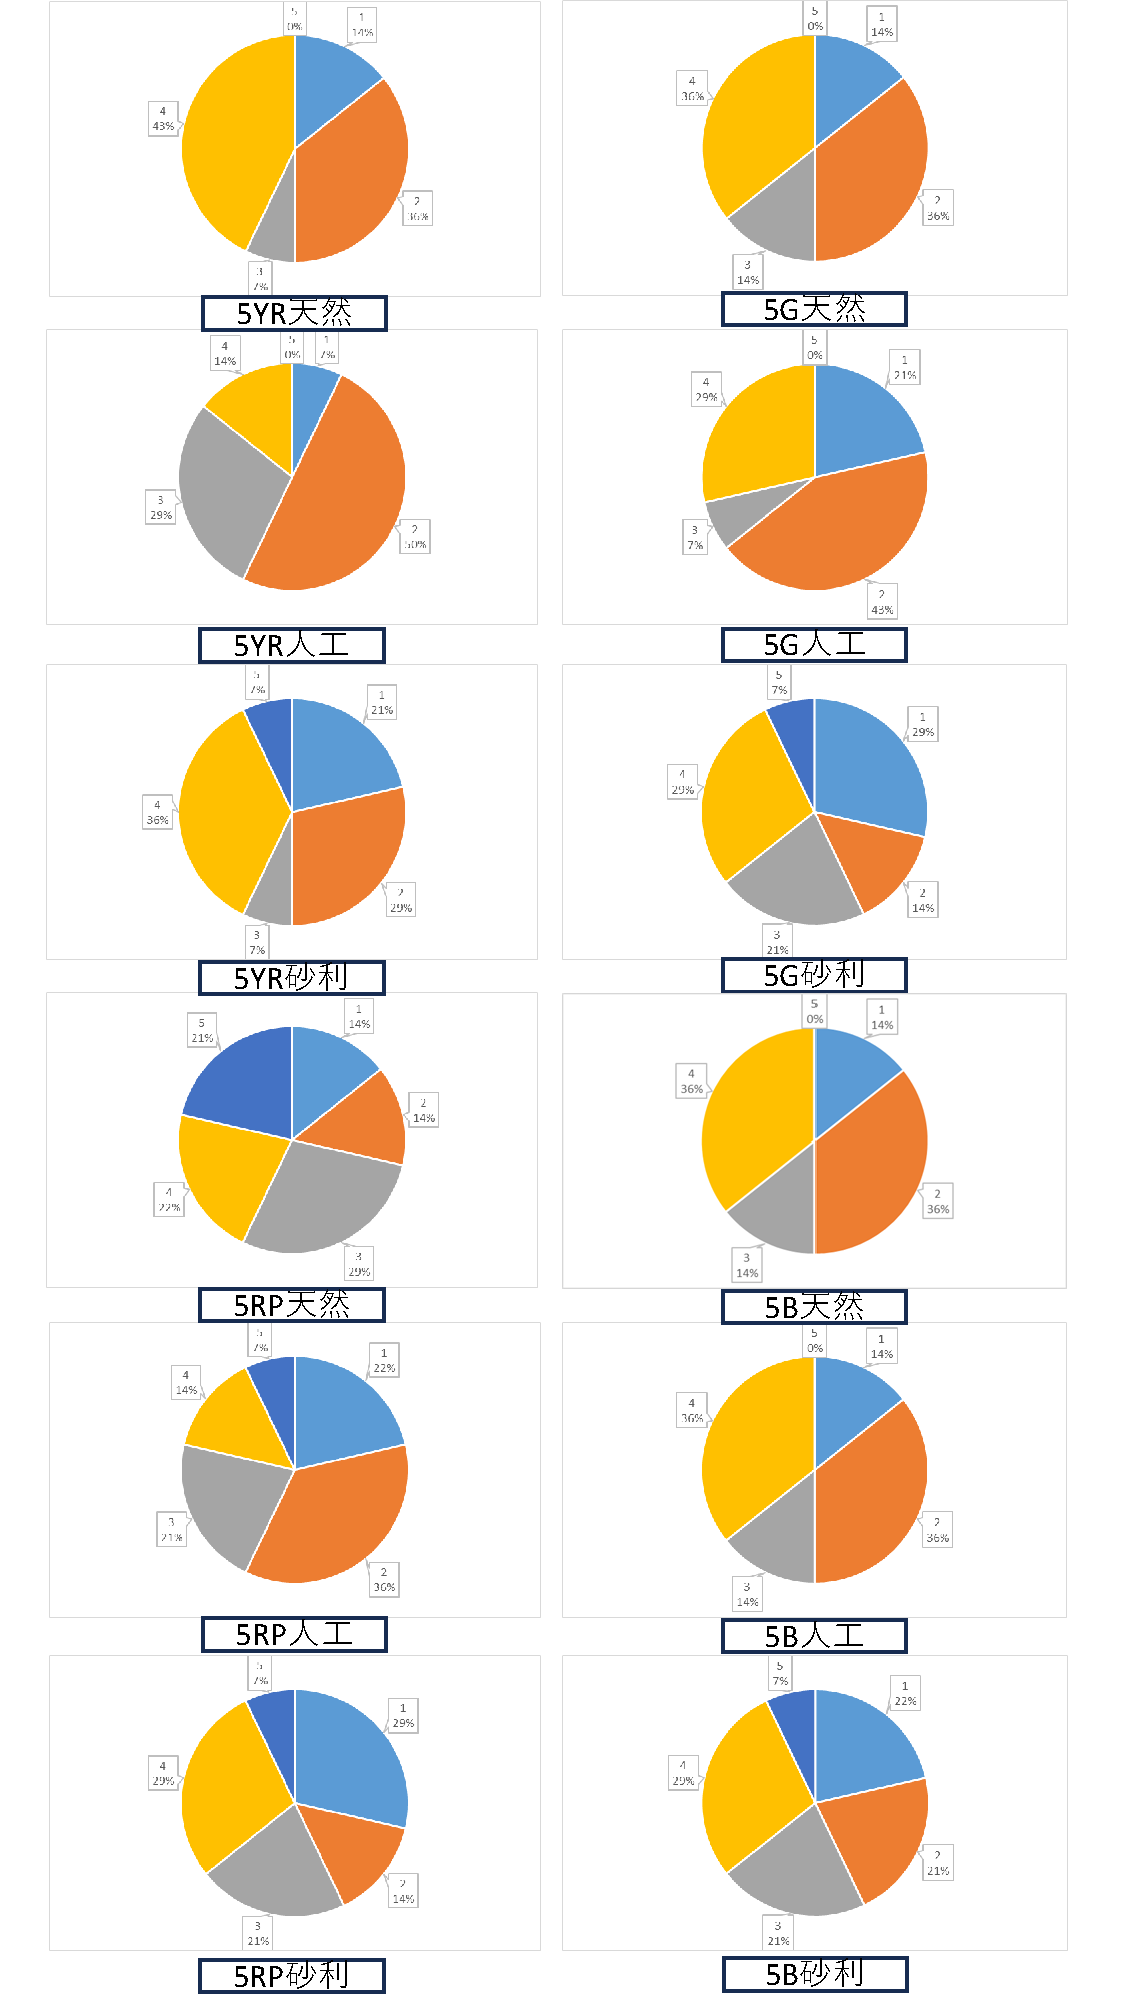
\includegraphics[width=0.8\linewidth]{fig/similar.pdf}
    }
    \caption{バーチャル床は本物の床が動いているように見えたかのアンケート結果}
    \label{fig:simi}
\end{figure}

\begin{figure}[H]
    \centering
    \fbox{
        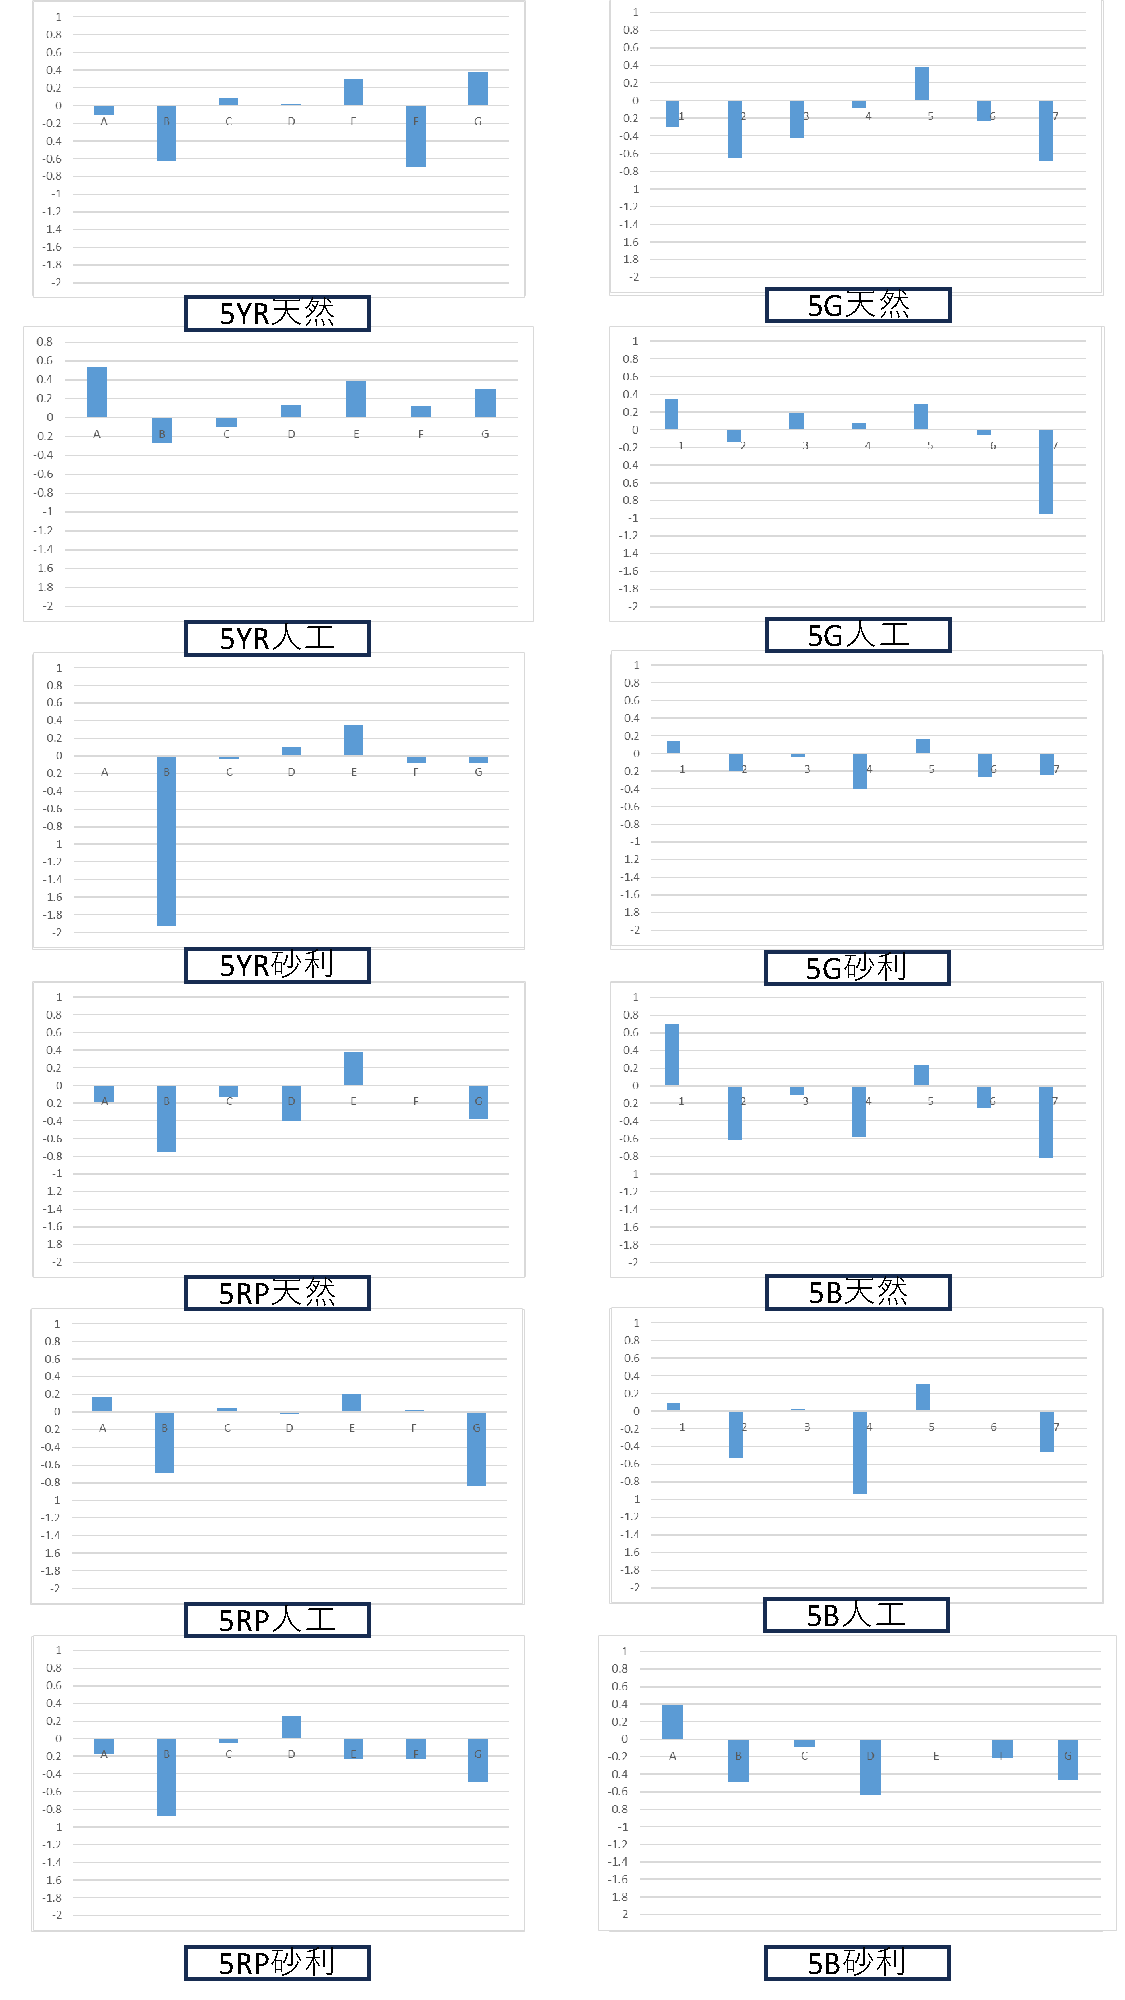
\includegraphics[width=0.8\linewidth]{fig/(前)halftime.pdf}
    }
    \caption{システム未使用時とシステム(前から迫ってくる)使用時の中間地点までの時間差一覧}
    \label{fig:maehalf}
\end{figure}
\begin{figure}[H]
    \centering
    \fbox{
        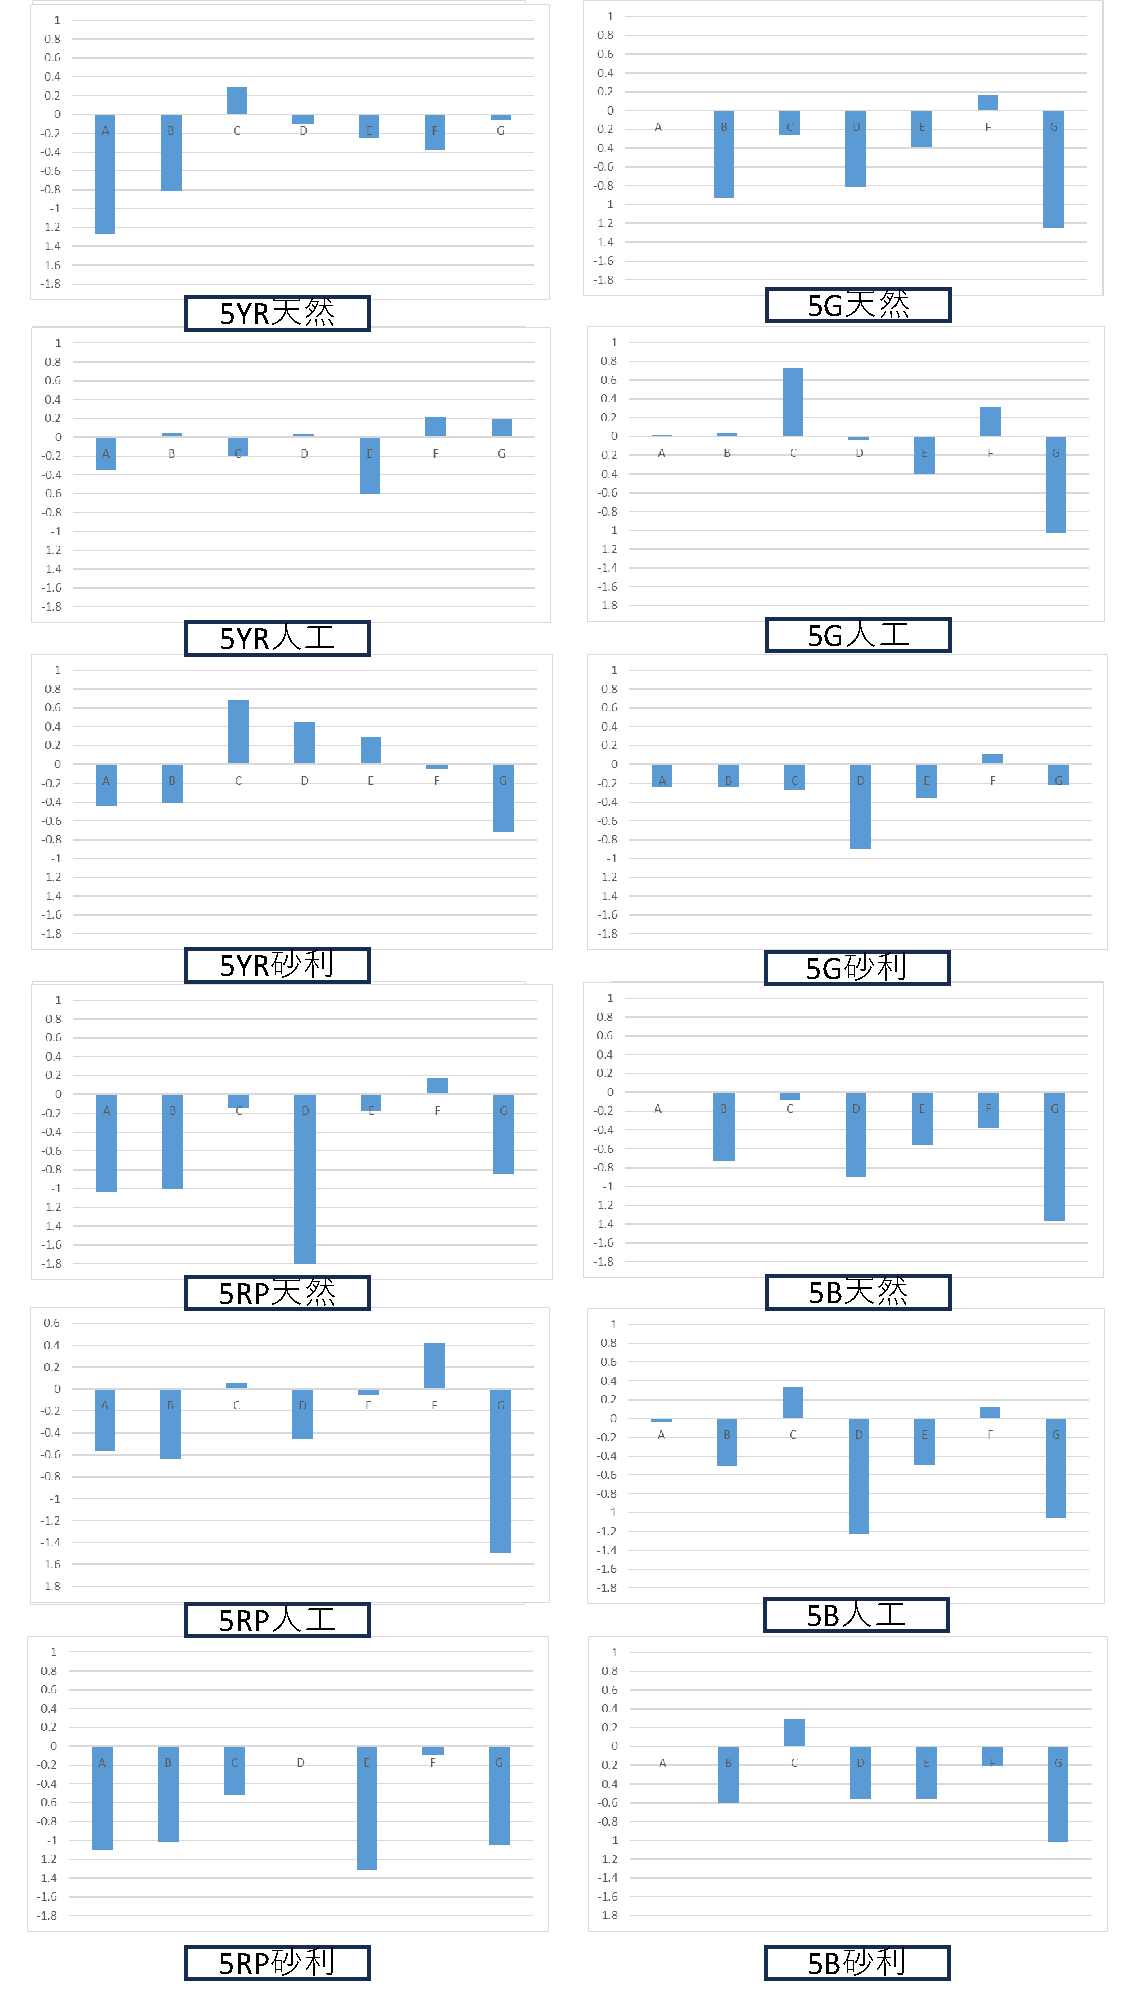
\includegraphics[width=0.8\linewidth]{fig/(前)time.pdf}
    }
    \caption{システム未使用時とシステム(前から迫ってくる)使用時のゴールまでの時間差一覧}
    \label{fig:maetime}
\end{figure}
\begin{figure}[H]
    \centering
    \fbox{
        \includegraphics[width=0.8\linewidth]{fig/(後)halftime.pdf}
    }
    \caption{システム未使用時とシステム(後ろから追い越してくる)使用時の中間地点までの時間差一覧}
    \label{fig:usirohalf}
\end{figure}
\begin{figure}[H]
    \centering
    \fbox{
        \includegraphics[width=0.8\linewidth]{fig/(後)time.pdf}
    }
    \caption{システム未使用時とシステム(後ろから追い越してくる)使用時のゴールまでの時間差一覧}
    \label{fig:usirotime}
\end{figure}